\documentclass[11pt]{article}
\usepackage{graphicx}
\usepackage{amsmath,amssymb,amsthm}
\usepackage{float}
\usepackage{booktabs}
\usepackage[margin=1in]{geometry}
\usepackage{placeins}
\usepackage{algorithm}
\usepackage{algpseudocode}
\usepackage{subcaption}
\usepackage[font=small]{caption}
\usepackage{listings}
\usepackage{xcolor}

\graphicspath{{../results/}}
\captionsetup[table]{position=top}

\setlength{\textfloatsep}{10pt plus 2pt minus 2pt}
\setlength{\floatsep}{8pt plus 2pt minus 2pt}
\setlength{\intextsep}{8pt plus 2pt minus 2pt}

\lstdefinestyle{pycode}{
  language=Python,
  basicstyle=\ttfamily\footnotesize,
  keywordstyle=\color{blue!70!black},
  commentstyle=\color{green!40!black},
  stringstyle=\color{orange!60!black},
  numbers=left,
  numberstyle=\tiny\color{gray},
  stepnumber=1,
  numbersep=8pt,
  showstringspaces=false,
  breaklines=true,
  frame=single
}

\newtheorem{proposition}{Proposition}

\title{Decentralized Smart EV Charging}
\author{Xiangyu LUO}
\date{January 2026}

\begin{document}
\maketitle
\tableofcontents
\clearpage

\section{Model and Game Analysis}
\label{sec:model_game}

We consider one day split into $T=48$ half-hour slots ($\delta=0.5$ h). For each EV $j\in\{1,\dots,J\}$, $\ell^{\mathrm{EV}}_j(t)$ is charging power (kW) at slot $t$. Let $\tilde \ell_{\mathrm{NF}}(t)$ be the non-flexible load forecast and define total load
\[
L(t)=\tilde \ell_{\mathrm{NF}}(t)+\sum_{m=1}^J \ell^{\mathrm{EV}}_m(t).
\]
The CO$_2$ objective uses the convex piecewise-linear function $f_{\mathrm{CO}_2}(\cdot)$ derived from the merit-order approximation in the reference document.

\subsection{Merit-Order Formulation of the CO$_2$ Function}
\label{subsec:piecewise_design}

The CO$_2$ model follows a merit-order approximation in five steps: define effective capacities, sort assets by variable cost (tie-break by emission rate), build cumulative breakpoints, assign each load increment to its active segment, and aggregate segment emissions. Let $P_i^{\mathrm{name}}$ be the installed capacity of asset $i$ and define effective capacities
\[
P_i=\kappa_i P_i^{\mathrm{name}},
\]
with $\kappa_i=0.3$ for wind, $\kappa_i=0.2$ for solar, $\kappa_i=\nu$ for nuclear (availability factor), and $\kappa_i=1$ otherwise. After sorting, cumulative breakpoints are
\[
\hat P_i:=\sum_{k=1}^i P_k,\qquad \hat P_0:=0.
\]
For demand level $\ell$ (MW), the dispatched quantity on segment $i$ is
\[
q_i(\ell):=\min\{P_i,\,[\ell-\hat P_{i-1}]_+\}
=\left[\min\{\ell,\hat P_i\}-\hat P_{i-1}\right]_+.
\]
Let $r_i$ be combustion emission rates (gCO$_2$eq/kWh) and define cumulative rates
\[
\gamma_i:=\sum_{k=1}^i r_k,\qquad \gamma_0:=0.
\]
The hourly emission score implemented in code is the piecewise-linear map
\begin{equation}
\label{eq:fco2_piecewise}
f_{\mathrm{CO}_2}(\ell)
=1000\sum_{i=1}^{I}\gamma_i\,q_i(\ell),
\end{equation}
where $[\cdot]_+=\max(\cdot,0)$. On interval $\ell\in[\hat P_{i-1},\hat P_i]$, the slope is $1000\gamma_i$. Since all $r_i\ge 0$, the sequence $(\gamma_i)$ is nondecreasing, which gives convexity. The factor 1000 converts MW to kW, so $f_{\mathrm{CO}_2}$ is in gCO$_2$eq/h.

Equation~\eqref{eq:fco2_piecewise} is a broken-line function with slope changes at breakpoints $(\hat P_i)$. In code, assets are first sorted; then cumulative capacities (\texttt{p\_hat}) and cumulative rates are built before segment-wise accumulation (Appendix~A).

Daily emissions are then computed by time aggregation:
\[
\mathrm{CO2}_{\mathrm{day}}=\sum_{t=1}^{48}f_{\mathrm{CO}_2}(L(t))\,\delta,\qquad \delta=0.5\text{ h}.
\]
Capacity-factor and availability assumptions are therefore embedded directly in the breakpoints and are consistently reused in the sensitivity analysis.

\begin{figure}[H]
\centering
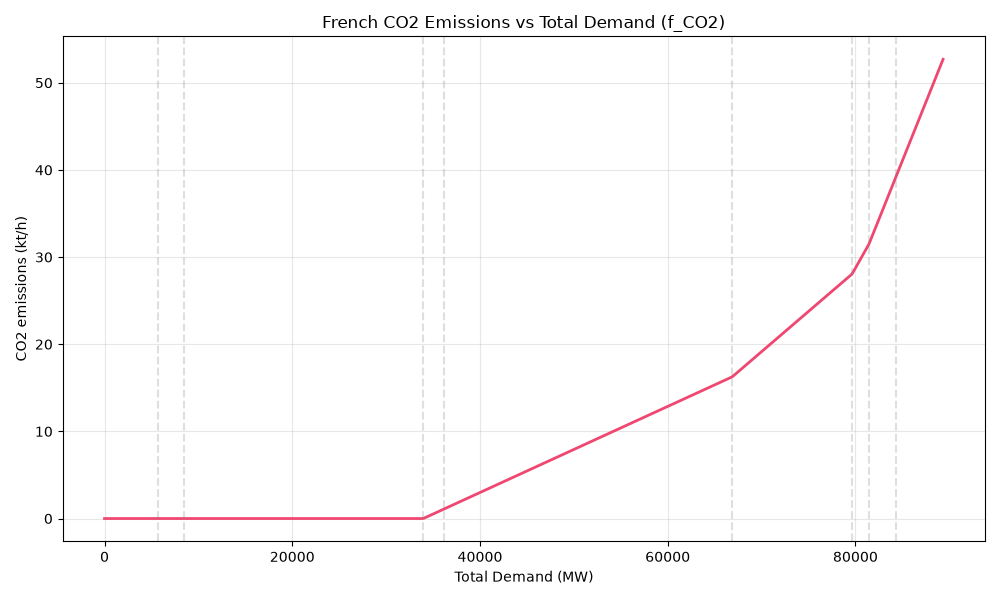
\includegraphics[width=0.82\linewidth]{f_co2_curve.png}
\caption{Piecewise-linear approximation of $f_{\mathrm{CO}_2}(L)$.}
\label{fig:f_co2_curve}
\end{figure}

\subsection{Individual EV Optimization}
\label{subsec:individual_problem}

Given the profiles of other EVs, EV $j$ solves
\begin{equation}
\label{eq:Pj}
\mathcal P_j:\quad
\min_{\ell^{\mathrm{EV}}_j}
\sum_{t=1}^{T} f_{\mathrm{CO}_2}\!\left(
\tilde \ell_{\mathrm{NF}}(t) + \sum_{m\neq j}\ell^{\mathrm{EV}}_m(t)+\ell^{\mathrm{EV}}_j(t)
\right)
\quad
\text{s.t. }\;
\big(\ell^{\mathrm{EV}}_j(t)\big)_{t=1}^{T}\in \mathcal L_j.
\end{equation}

The feasible set is
\begin{equation}
\label{eq:Lj}
\mathcal L_j=
\left\{
(\ell^{\mathrm{EV}}_j(t))_{t=1}^T:
\begin{array}{l}
\ell^{\mathrm{EV}}_j(t)=0 \;\text{for } t\notin\{a_j+1,\dots,d_j-1\},\\
0\le \ell^{\mathrm{EV}}_j(t)\le 7 \;\text{for } t\in\{a_j+1,\dots,d_j-1\},\\
\sum_{t=a_j+1}^{d_j-1}\ell^{\mathrm{EV}}_j(t)=\dfrac{e_j}{\delta}.
\end{array}
\right\}.
\end{equation}

Since $f_{\mathrm{CO}_2}$ is convex and the constraints are affine plus box bounds, each individual problem is convex (possibly non-smooth at breakpoints).

The EV objective is written in terms of system-level emissions, not only private charging convenience. In that sense, the player-level optimization is aligned with the global objective. This alignment yields favorable equilibrium properties, but it is also a normative modeling choice rather than a purely behavioral one.

At system scale, one vehicle has negligible unilateral influence: its maximum charging power (7 kW) is around $10^{-7}$ of a 60--70 GW national load level. Hence, in isolation, one EV cannot materially modify the emission trajectory. The relevance emerges only at fleet level, where coordinated responses produce non-negligible aggregate load shifts.

\subsection{Water-Filling Optimality and Implementation}
\label{subsec:water_filling}

Fix
\[
b(t):=\tilde \ell_{\mathrm{NF}}(t)+\sum_{m\neq j}\ell^{\mathrm{EV}}_m(t),
\]
and define $x(t):=\ell^{\mathrm{EV}}_j(t)$ on $\mathcal T_j=\{a_j+1,\dots,d_j-1\}$. Then
\begin{equation}
\label{eq:Pj_simplified}
\min_{x}\; \sum_{t\in\mathcal T_j} f_{\mathrm{CO}_2}(b(t)+x(t))
\quad\text{s.t.}\quad
0\le x(t)\le P_{\max},\ \sum_{t\in\mathcal T_j}x(t)=E,
\end{equation}
with $P_{\max}=7$ kW and $E=e_j/\delta$.

At optimum $x^\star$, there exist $\lambda\in\mathbb R$ and nonnegative multipliers $\mu_t^-,\mu_t^+$ such that
\begin{equation}
\label{eq:KKT_subgrad}
0\in \partial f_{\mathrm{CO}_2}(b(t)+x^\star(t)) + \lambda - \mu_t^- + \mu_t^+,
\qquad
\mu_t^-x^\star(t)=0,
\ \mu_t^+(P_{\max}-x^\star(t))=0.
\end{equation}
Thus, interior active slots equalize marginal cost levels; with increasing slopes, energy must be allocated first on the currently lowest-load slots.

An equivalent exchange argument is immediate: if $L_1<L_2$ with $x_2>0$ and $x_1<P_{\max}$, shifting an infinitesimal charge from slot 2 to slot 1 does not increase objective value by convexity.

The implemented heuristic exactly follows this logic.

\begin{algorithm}[H]
\caption{Water-Filling Best Response for One EV}
\label{alg:water_filling}
\begin{algorithmic}[1]
\Require EV parameters $(a_j,d_j,e_j)$, baseline load $b(t)$, increment $\epsilon$, maximum iterations $K$
\Ensure Charging profile $x_j(t)$
\State Initialize $x_j(t)\gets 0$ for all $t\in\{1,\dots,48\}$
\State $E\gets e_j/\delta$, $k\gets 0$
\While{$k<K$ \textbf{and} $\sum_t x_j(t)<E$}
    \State $k\gets k+1$
    \State $\mathcal T_{\mathrm{nonsat}}\gets\{t\in\{a_j+1,\dots,d_j-1\}: x_j(t)<7\}$
    \If{$\mathcal T_{\mathrm{nonsat}}=\varnothing$}
        \State \textbf{break}
    \EndIf
    \State $\mathcal T_{\min}\gets\arg\min_{t\in\mathcal T_{\mathrm{nonsat}}}\big(b(t)+x_j(t)\big)$
    \State $\Delta\gets \min\!\left(\epsilon,\dfrac{E-\sum_t x_j(t)}{|\mathcal T_{\min}|}\right)$
    \ForAll{$t\in\mathcal T_{\min}$}
        \State $x_j(t)\gets\min\{x_j(t)+\Delta,7\}$
    \EndFor
\EndWhile
\end{algorithmic}
\end{algorithm}

\subsection{Potential Game Structure and BRD Update}
\label{subsec:potential_structure}

Define the social potential
\begin{equation}
\label{eq:Phi}
\Phi(\ell^{\mathrm{EV}}_1,\dots,\ell^{\mathrm{EV}}_J)
:= \sum_{t=1}^{T} f_{\mathrm{CO}_2}\!\left(\tilde \ell_{\mathrm{NF}}(t)+\sum_{m=1}^J \ell^{\mathrm{EV}}_m(t)\right).
\end{equation}
For fixed $\ell_{-j}$, player $j$ minimizes $\Phi(\ell_j,\ell_{-j})$. The game is therefore an exact potential game and, more specifically, a team game.

The BRD procedure implemented in this work is reported below.

\begin{algorithm}[H]
\caption{Best-Response Dynamics (BRD)}
\label{alg:brd}
\begin{algorithmic}[1]
\Require EV set $\{1,\dots,J\}$, non-flexible load $L_{\mathrm{nf}}(t)$, fleet scaling factor $\alpha$, threshold $\eta$, max iterations $K$
\Ensure Charging profiles $p_j(t)$
\State Initialize $p_j(t)=0$ for all $j,t$; initialize aggregate EV load $L_{\mathrm{EV}}(t)=0$
\For{$k=1$ to $K$}
    \State Store previous profiles $p_j^{\mathrm{prev}}(t)$
    \ForAll{$j\in\{1,\dots,J\}$}
        \State $L_{\mathrm{base}}(t)\gets L_{\mathrm{nf}}(t)+\alpha\cdot\big(L_{\mathrm{EV}}(t)-p_j(t)\big)$
        \State $p_j(t)\gets$ Water-Filling best response of EV $j$ under $L_{\mathrm{base}}(t)$
        \State $L_{\mathrm{EV}}(t)\gets L_{\mathrm{EV}}(t)-p_j^{\mathrm{prev}}(t)+p_j(t)$
    \EndFor
    \State $\mathrm{diff}\gets\sum_{j=1}^J\|p_j-p_j^{\mathrm{prev}}\|_2^2$
    \If{$\mathrm{diff}<\eta$}
        \State \textbf{break}
    \EndIf
\EndFor
\end{algorithmic}
\end{algorithm}

Each block update cannot increase $\Phi$, so BRD is a cyclic block-coordinate descent on a convex potential.

\subsection{PoA, Existence, and Non-Uniqueness}
\label{subsec:poa_equilibria}

Let $\mathcal L=\mathcal L_1\times\cdots\times\mathcal L_J$ and $\mathrm{NE}$ denote the Nash equilibria. Define
\[
\mathrm{OPT}=\min_{\ell\in\mathcal L}\Phi(\ell),
\qquad
\mathrm{PoA}=\frac{\max_{\ell\in\mathrm{NE}}\Phi(\ell)}{\min_{\ell\in\mathcal L}\Phi(\ell)}.
\]

\begin{proposition}[PoA equals 1 under exact best responses]
\label{prop:poa1}
Assume $\Phi$ is convex and $\mathcal L=\mathcal L_1\times\cdots\times\mathcal L_J$ is nonempty, convex, and compact. If each player computes an exact best response of $\Phi(\ell_j,\ell_{-j})$ over $\mathcal L_j$, then every Nash equilibrium is globally optimal and $\mathrm{PoA}=1$.
\end{proposition}

\begin{proof}
At equilibrium, each block $j$ is optimal given $\ell_{-j}$:
\[
\Phi(\ell_j^\star,\ell_{-j}^\star)\le \Phi(\ell_j,\ell_{-j}^\star),\quad \forall \ell_j\in\mathcal L_j.
\]
For each block problem (convex objective, convex feasible set), first-order optimality gives
\[
0\in \partial_j\Phi(\ell^\star)+N_{\mathcal L_j}(\ell_j^\star),\quad j=1,\dots,J,
\]
where $N_{\mathcal L_j}$ is the normal cone. Because $\mathcal L=\mathcal L_1\times\cdots\times\mathcal L_J$, stacking these inclusions yields
\[
0\in \partial\Phi(\ell^\star)+N_{\mathcal L}(\ell^\star).
\]
For a convex objective on a convex feasible set, this first-order condition is sufficient for global optimality. Hence $\ell^\star$ solves $\min_{\ell\in\mathcal L}\Phi(\ell)$ and attains $\mathrm{OPT}$.
\end{proof}

Existence follows from continuity of $\Phi$ and compactness of $\mathcal L$. Uniqueness of the objective value is guaranteed, but uniqueness of schedules is not, because $f_{\mathrm{CO}_2}$ is piecewise linear and $\Phi$ is generally not strictly convex. BRD may converge to different profiles with the same final CO$_2$ score.

\subsection{Information Structure and Practical Interpretation}
\label{subsec:information_structure}

The optimization of EV $j$ depends on
\[
b_j(t)=\tilde \ell_{\mathrm{NF}}(t)+\sum_{m\ne j}\ell_m^{\mathrm{EV}}(t),
\]
which is an aggregate quantity. Therefore, the mechanism does not require each EV to observe all individual neighbor schedules. This aggregate-only dependency is consistent with a privacy-preserving decentralized implementation.

However, practical deployment still requires communication infrastructure and trusted signal generation. In operational terms, an aggregator (or system operator) must broadcast a reliable aggregate baseline or equivalent marginal signal; agents then solve local updates against this signal. Forecast error and delayed information can affect convergence speed and final quality, even if the static model predicts strong optimality properties.

\section{Experimental Setup}
\label{sec:setup}

\subsection{Scenario and Policy Configuration}
\label{subsec:scenario_policy}

The experiments cover summer/winter conditions in 2019 and 2020. A simulated set of $J=500$ EVs is scaled to a fleet of $N=15$ million EVs. The charging policies are summarized in Table~\ref{tab:policies}.

\begin{table}[H]
\centering
\caption{Charging policies used in the experiments.}
\label{tab:policies}
\begin{tabular}{p{0.27\linewidth}p{0.66\linewidth}}
\toprule
\textbf{Policy} & \textbf{Implementation rule} \\
\midrule
Plug-and-Charge (PC) & Charging starts immediately after arrival, up to 7 kW, until energy need is met. \\
Off-Peak (OP) & Start time is drawn uniformly (seeded) in the off-peak window (22:00 to 06:00), then charging proceeds at up to 7 kW. \\
Off-Peak, synchronized (OP-22) & Every EV starts at 22:00, the literal off-peak tariff signal, at up to 7 kW. Used as a herding stress test in the load-shape and threshold diagnostics. \\
Smart Charging (BRD) & Sequential best-response updates with Water-Filling as per-EV optimizer. \\
\bottomrule
\end{tabular}
\end{table}

\subsection{Evaluation Procedure}
\label{subsec:evaluation_procedure}

The global simulation workflow is the following.

\begin{algorithm}[H]
\caption{Policy Evaluation Workflow}
\label{alg:policy_eval}
\begin{algorithmic}[1]
\Require Scenario $(y,s)$, EV scenario set, baseline load $L_{\mathrm{nf}}(t)$, fleet size $N$, simulation size $N_{\mathrm{sim}}$
\Ensure Policy-level emission scores and load curves
\State Load $L_{\mathrm{nf}}(t)$ and EV arrivals/departures/energy needs
\State Set scaling factor $\alpha\gets N/N_{\mathrm{sim}}$
\State Construct merit-order CO$_2$ model $f_{\mathrm{CO}_2}$
\ForAll{$P\in\{$PC, OP, BRD$\}$}
    \State Compute individual charging profiles under policy $P$
    \State Aggregate EV load and total load
    \State Evaluate total emissions $\sum_t f_{\mathrm{CO}_2}(L_{\mathrm{tot}}^P(t))\,\delta$
\EndFor
\State Export aggregated indicators and figures
\end{algorithmic}
\end{algorithm}

\section{Numerical Results}
\label{sec:results}

\subsection{Convergence of BRD}
\label{subsec:convergence_results}

Table~\ref{tab:brd_iterations} shows that BRD converges in 3 to 7 sweeps depending on scenario, with small final move norms. This confirms that most of the useful adjustment happens in early iterations. The scenario dependence is meaningful: cases with flatter low-load periods tend to require more redistribution steps before the stopping criterion is reached.

Figure~\ref{fig:brd_convergence} provides the dynamic view. The first sweeps produce the steepest drop, indicating rapid elimination of inefficient charging placements. The tail of the curve is much flatter, which is expected under a convex but non-strictly convex potential: late updates mainly reallocate charging among nearly equivalent slots with very small objective improvements.

\begin{table}[H]
\centering
\caption{BRD stopping statistics by scenario.}
\label{tab:brd_iterations}
\begin{tabular}{lcc}
\toprule
\textbf{Scenario} & \textbf{BRD iterations} & \textbf{Final move norm} \\
\midrule
2019 Summer & 5 & 0.145083 \\
2019 Winter & 3 & 0.618738 \\
2020 Summer & 7 & 0.718181 \\
2020 Winter & 4 & 0.117583 \\
\bottomrule
\end{tabular}
\end{table}

\begin{figure}[H]
\centering
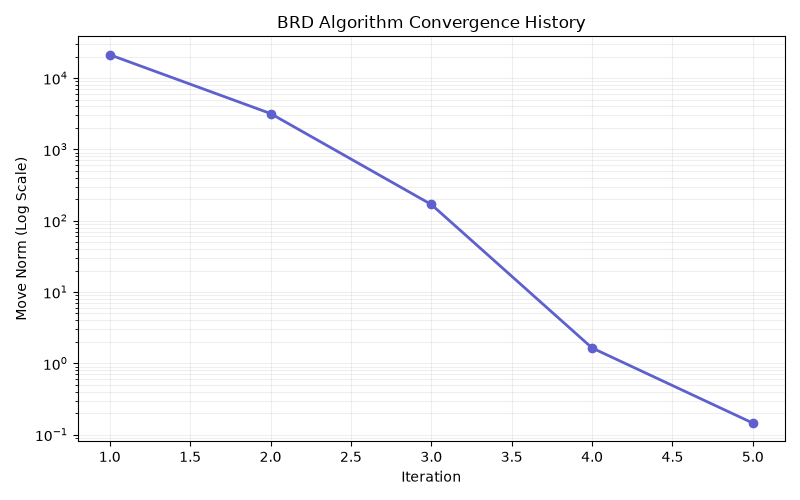
\includegraphics[width=0.90\linewidth]{brd_convergence.png}
\caption{BRD convergence trajectory.}
\label{fig:brd_convergence}
\end{figure}
\FloatBarrier

\subsection{Emission Performance by Policy}
\label{subsec:co2_performance}

Table~\ref{tab:co2_merged} reports absolute daily emissions and relative gains in a single view. Three findings emerge.

First, BRD is never worse than the alternatives and is strictly better than PC in every scenario. The reduction reaches 16.03\% in 2019 winter and 15.16\% in 2020 winter.

Second, OP is beneficial compared with PC but systematically dominated by BRD in winter and 2020 summer. The BRD-over-OP gain is substantial in winter: about 19,593 tons/day in 2019 winter and 19,946 tons/day in 2020 winter. In 2020 summer the gain is smaller (about 3,202 tons/day), consistent with a lower average marginal carbon intensity.

Third, 2019 summer is a boundary case where OP and BRD are numerically identical at the reported precision. This indicates that in that low-stress regime, a simple off-peak shift can already place most EV energy on low-carbon merit-order segments, leaving little room for additional optimization.
\begin{table}[H]
\centering
\caption{Policy-level CO$_2$ performance by scenario.}
\label{tab:co2_merged}
\small
\begin{tabular}{ccrrrrrr}
\toprule
\textbf{Year} & \textbf{Season} & \textbf{PC (t)} & \textbf{OP (t)} & \textbf{BRD (t)} & \textbf{OP vs. PC} & \textbf{BRD vs. PC} & \textbf{BRD vs. OP} \\
\midrule
2019 & Summer & 143,790 & 141,684 & 141,684 & 1.46\% & 1.46\% & 0.00\% \\
2019 & Winter & 395,700 & 351,850 & 332,257 & 11.08\% & 16.03\% & 5.57\% \\
2020 & Summer & 93,699 & 88,842 & 85,640 & 5.18\% & 8.60\% & 3.60\% \\
2020 & Winter & 470,941 & 419,486 & 399,541 & 10.93\% & 15.16\% & 4.75\% \\
\bottomrule
\end{tabular}
\normalsize
\end{table}

Figure~\ref{fig:co2_comparison} confirms these cross-scenario patterns visually: inter-policy spacing is narrow in summer, while winter bars are clearly separated, with BRD lowest.

\begin{figure}[H]
\centering
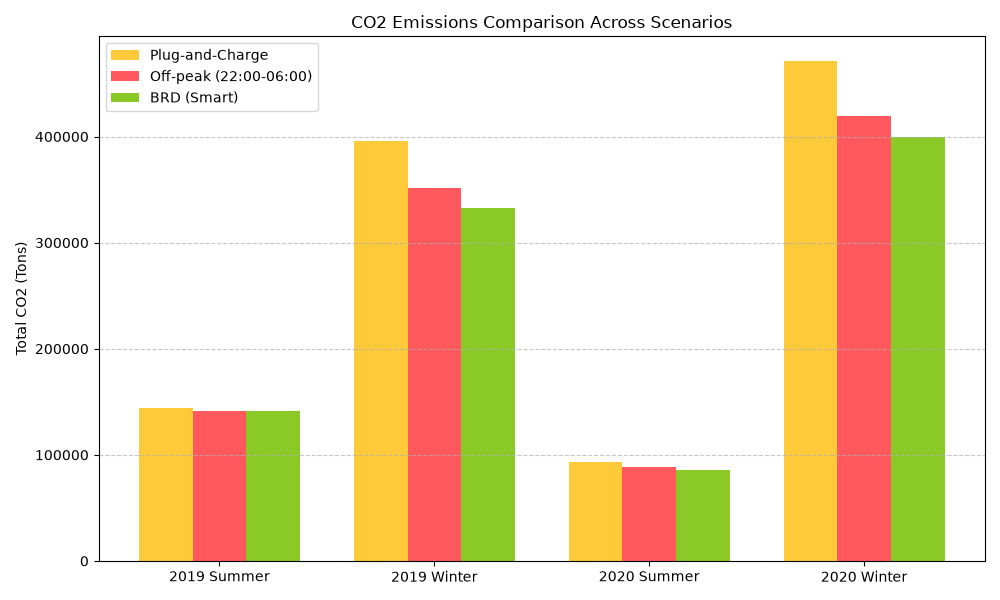
\includegraphics[width=0.88\linewidth]{co2_comparison.png}
\caption{Total CO$_2$ emissions by policy and scenario.}
\label{fig:co2_comparison}
\end{figure}

\subsection{Load-Shape Mechanisms Behind the Scores}
\label{subsec:load_shapes}

To align figures with the argument, we first analyze total-load trajectories, then EV-only profiles, and finally threshold exceedance metrics.

Figure~\ref{fig:load_2x2} shows total load for the four scenarios. Two systematic effects appear. PC shifts substantial energy toward early charging hours and raises evening-night peaks. OP displaces this peak into the night window; since start times are spread over eight hours its peak is lower than under PC, but charging is still placed by the clock rather than by the load level, so it piles up on the night hours regardless of where the valleys are. BRD produces the flattest trajectories and keeps the system near the low-to-intermediate load bands for longer periods.

\begin{figure}[H]
\centering
\begin{subfigure}[t]{0.48\linewidth}
\centering
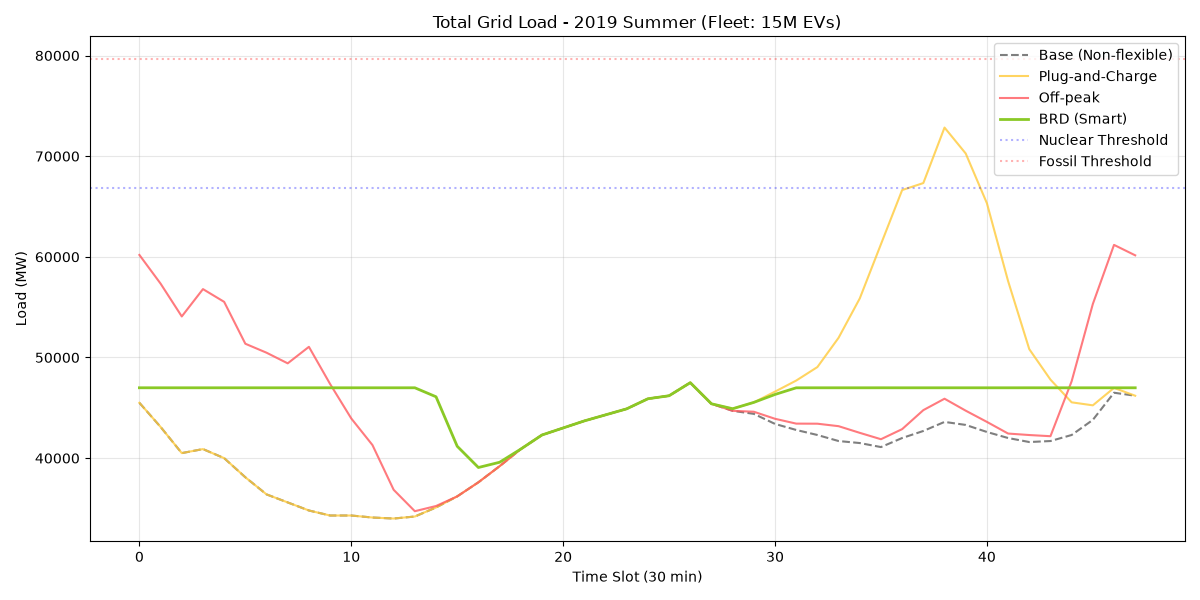
\includegraphics[width=\linewidth]{load_2019_summer.png}
\caption{2019 summer}
\end{subfigure}\hfill
\begin{subfigure}[t]{0.48\linewidth}
\centering
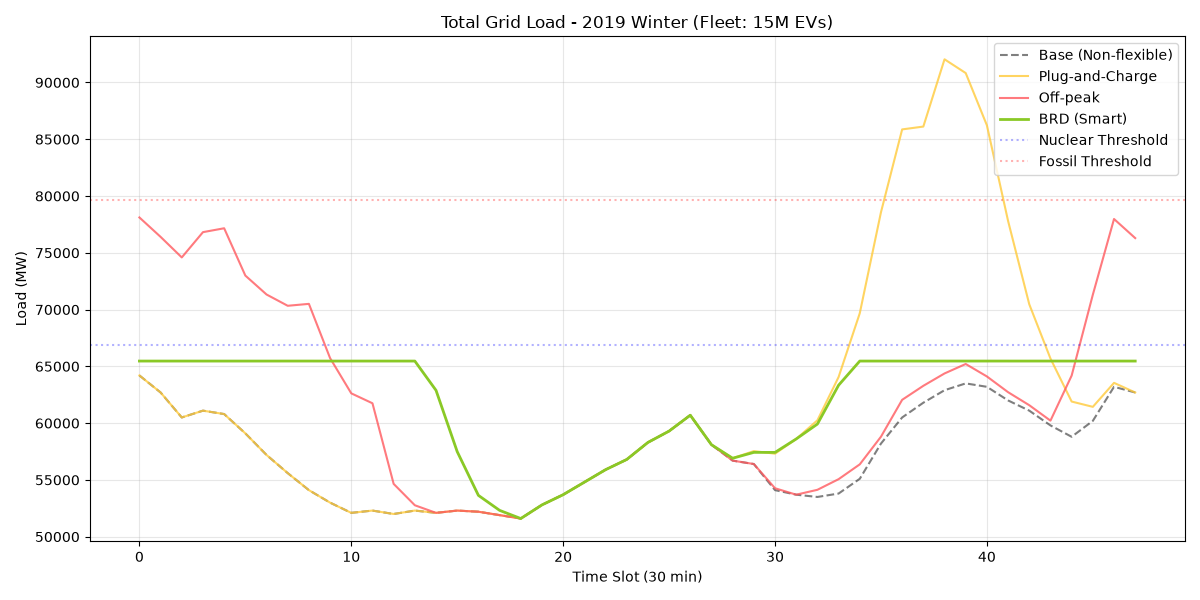
\includegraphics[width=\linewidth]{load_2019_winter.png}
\caption{2019 winter}
\end{subfigure}

\vspace{0.3em}

\begin{subfigure}[t]{0.48\linewidth}
\centering
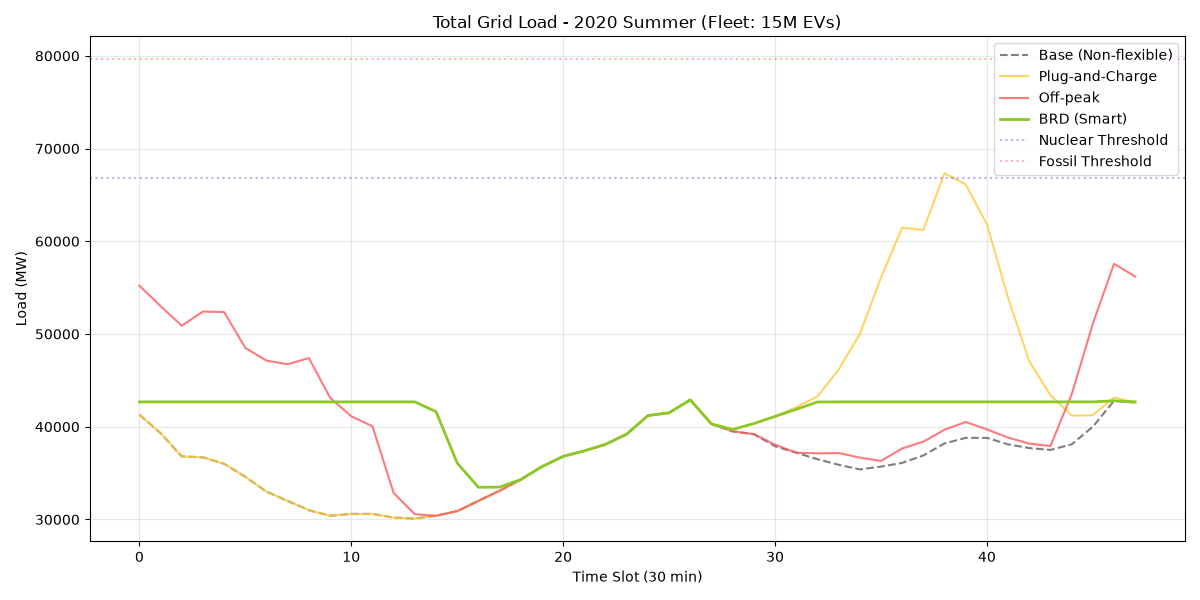
\includegraphics[width=\linewidth]{load_2020_summer.png}
\caption{2020 summer}
\end{subfigure}\hfill
\begin{subfigure}[t]{0.48\linewidth}
\centering
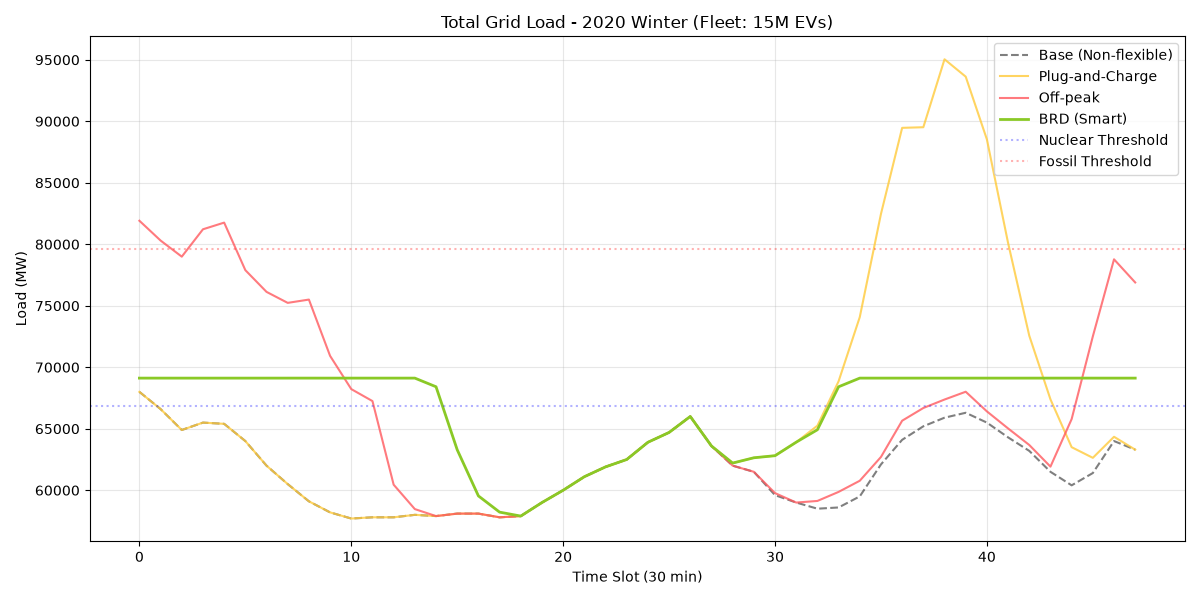
\includegraphics[width=\linewidth]{load_2020_winter.png}
\caption{2020 winter}
\end{subfigure}
\caption{Total grid load under PC, OP, and BRD across all scenarios.}
\label{fig:load_2x2}
\end{figure}

Table~\ref{tab:peak_load} quantifies this visual pattern. PC raises the base load peak by +40\% to +57\%. Randomized OP reduces this to +21\% to +34\%, whereas the synchronized variant OP-22, in which the whole fleet reacts to the same 22:00 signal, produces by far the largest peaks (+143\% to +234\%). BRD keeps peak growth near zero (0\% in both summer cases, about +2\% in winter). This is the central operational difference between coordinated valley filling and clock-synchronized charging.

\begin{table}[H]
\centering
\caption{Peak-load impact by scenario.}
\label{tab:peak_load}
\resizebox{\linewidth}{!}{%
\begin{tabular}{lrrrrrr}
\toprule
\textbf{Scenario} & \textbf{Base peak (MW)} & \textbf{PC peak (MW)} & \textbf{OP peak (MW)} & \textbf{OP-22 peak (MW)} & \textbf{BRD peak (MW)} & \textbf{BRD vs. base} \\
\midrule
2019 Summer & 47,500 & 72,844 & 61,188 & 147,300 & 47,500 & 0.00\% \\
2019 Winter & 64,200 & 92,042 & 78,114 & 163,800 & 65,468 & 1.98\% \\
2020 Summer & 42,900 & 67,342 & 57,578 & 143,100 & 42,900 & 0.00\% \\
2020 Winter & 68,000 & 95,042 & 81,914 & 165,400 & 69,118 & 1.64\% \\
\bottomrule
\end{tabular}
}
\end{table}

Figure~\ref{fig:ev_only_2x2} isolates EV demand. PC is front-loaded after arrivals; OP concentrates power around the off-peak window; BRD spreads charging over a wider feasible support. This explains why BRD lowers carbon cost even with identical total EV energy: it reallocates charging across time rather than reducing energy volume.

\begin{figure}[H]
\centering
\begin{subfigure}[t]{0.48\linewidth}
\centering
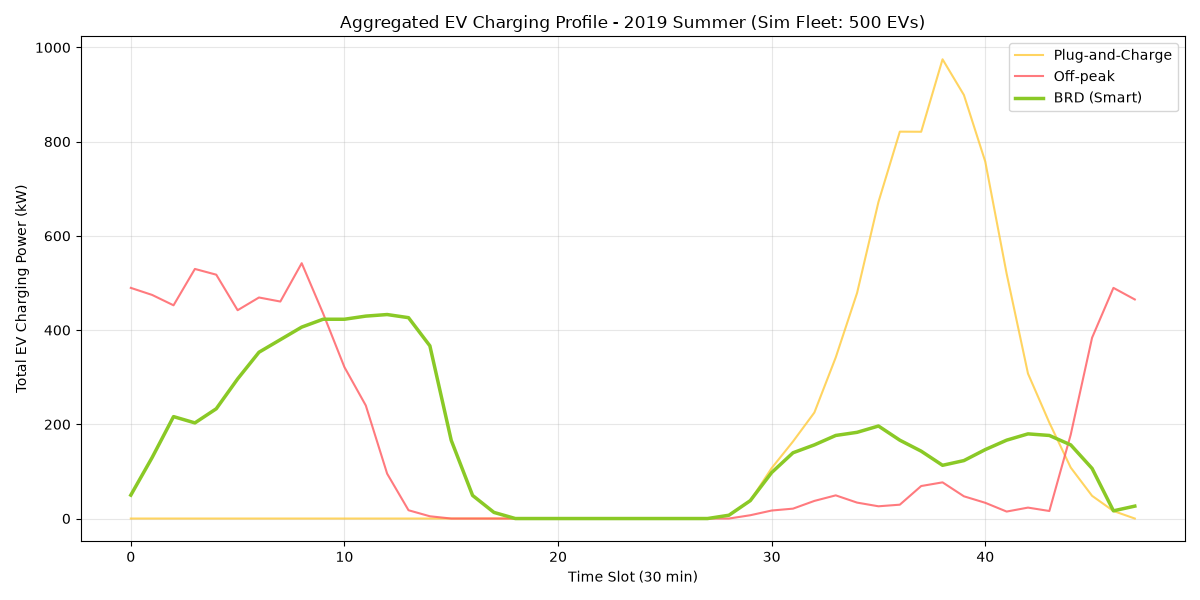
\includegraphics[width=\linewidth]{ev_only_2019_summer.png}
\caption{2019 summer}
\end{subfigure}\hfill
\begin{subfigure}[t]{0.48\linewidth}
\centering
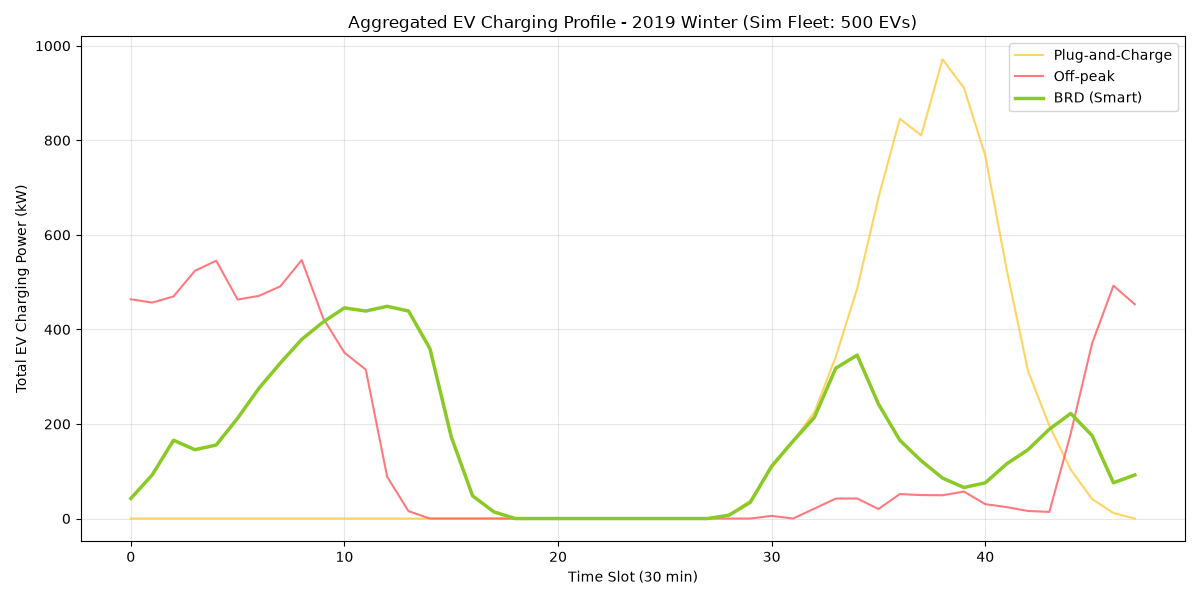
\includegraphics[width=\linewidth]{ev_only_2019_winter.png}
\caption{2019 winter}
\end{subfigure}

\vspace{0.3em}

\begin{subfigure}[t]{0.48\linewidth}
\centering
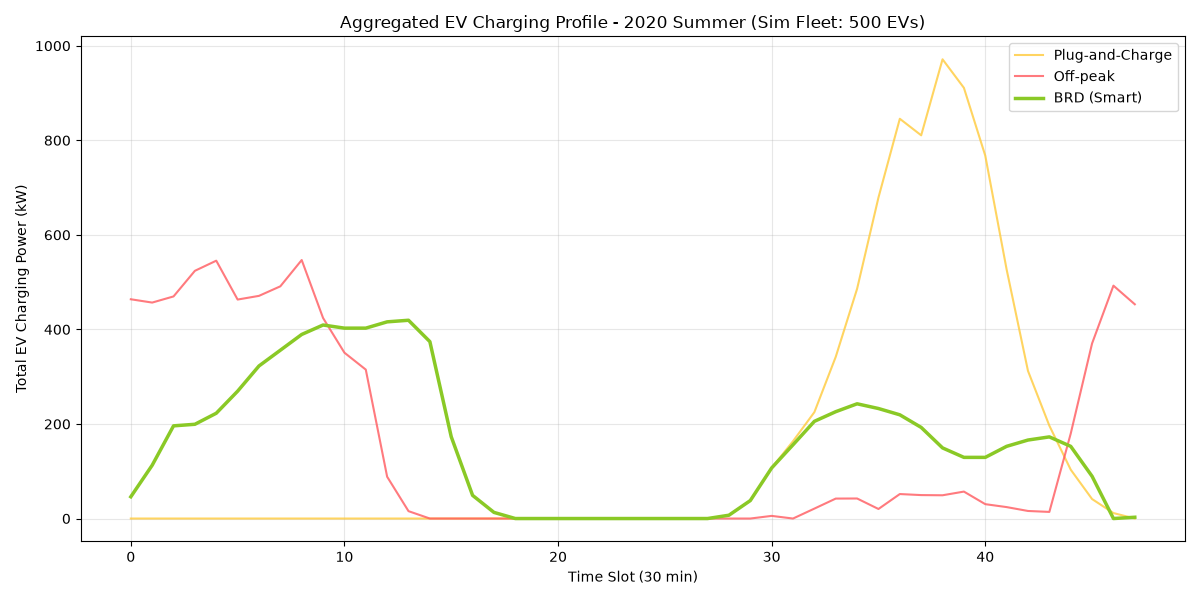
\includegraphics[width=\linewidth]{ev_only_2020_summer.png}
\caption{2020 summer}
\end{subfigure}\hfill
\begin{subfigure}[t]{0.48\linewidth}
\centering
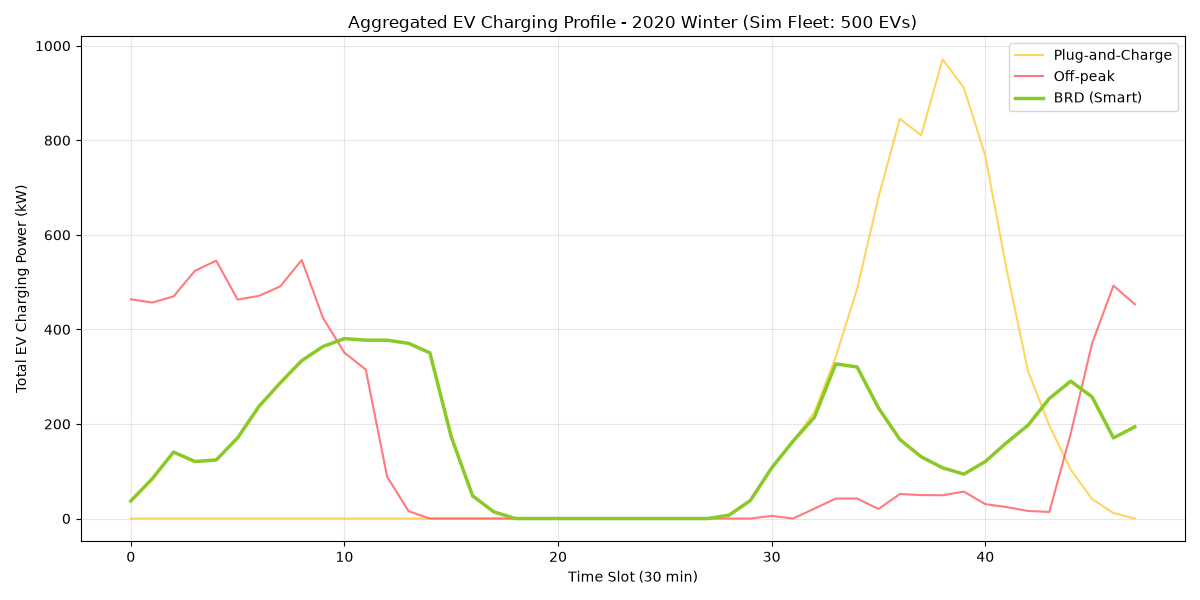
\includegraphics[width=\linewidth]{ev_only_2020_winter.png}
\caption{2020 winter}
\end{subfigure}
\caption{EV-only aggregate charging profiles.}
\label{fig:ev_only_2x2}
\end{figure}

Figure~\ref{fig:water_filling_2020_winter} provides a focused illustration of the BRD mechanism in winter. The optimized curve fills low-demand valleys first and creates a broad plateau rather than a narrow peak, which is precisely the geometry predicted by the KKT marginal-equalization argument in Section~\ref{subsec:water_filling}.

\begin{figure}[H]
\centering
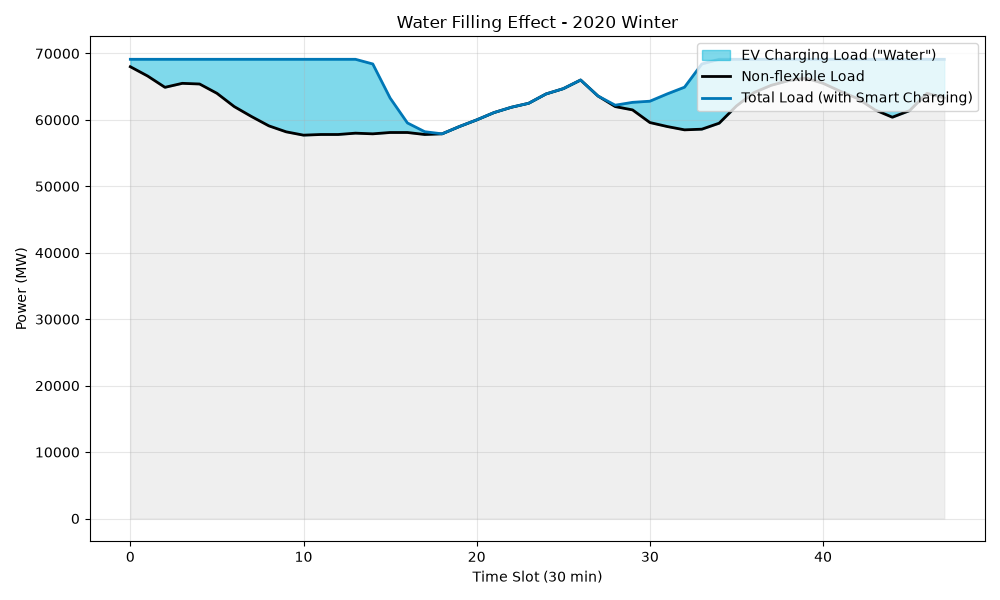
\includegraphics[width=0.92\linewidth]{water_filling_2020_winter.png}
\caption{Water-filling effect in 2020 winter.}
\label{fig:water_filling_2020_winter}
\end{figure}

Figure~\ref{fig:load_rebound_2020_winter} details the most constrained case (2020 winter). PC reaches the highest instantaneous peak (about 95 GW). OP reduces this specific peak (about 82 GW) but still crosses the gas threshold in several slots. BRD keeps the trajectory closer to the nuclear threshold and avoids gas-threshold crossing.

\begin{figure}[H]
\centering
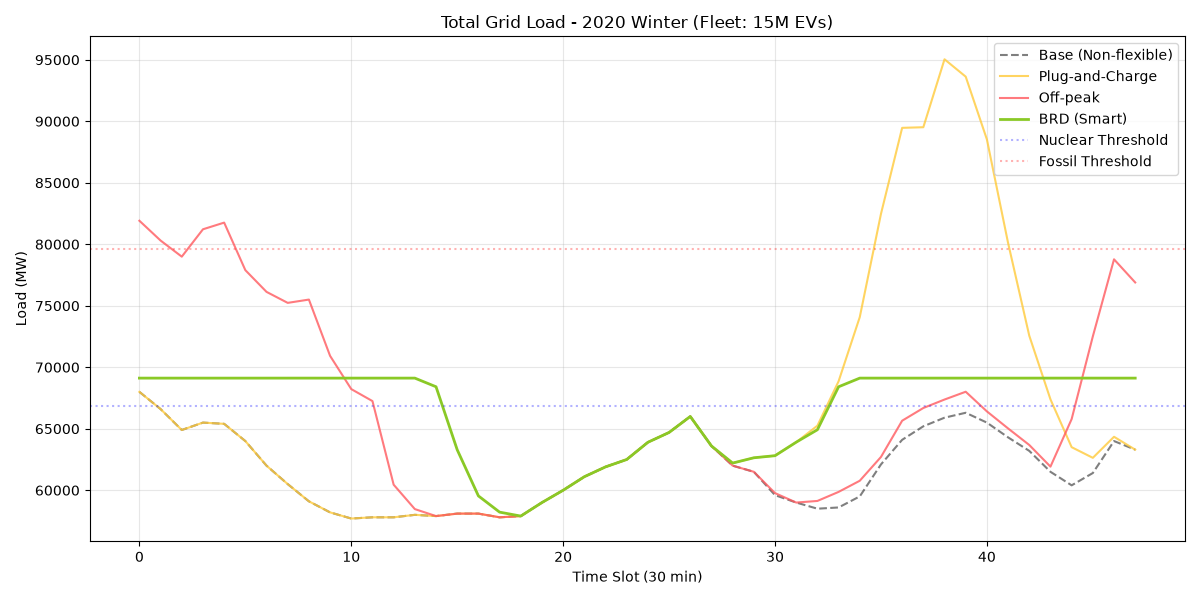
\includegraphics[width=0.95\linewidth]{load_2020_winter.png}
\caption{Detailed total-load comparison for 2020 winter.}
\label{fig:load_rebound_2020_winter}
\end{figure}

Table~\ref{tab:thresholds} confirms this across scenarios. The synchronized OP-22 policy exceeds the gas threshold in every scenario, randomized OP does so in 2020 winter, and BRD keeps gas exceedance at zero in all four scenarios. For nuclear-threshold exceedance, 2020 winter is instructive: BRD has more hours above threshold but much lower exceedance severity (32,935 MW-hours, against 71,028 for OP and 104,406 for OP-22), indicating flatter near-threshold operation instead of extreme spikes.

\begin{table}[H]
\centering
\caption{Threshold exceedance indicators.}
\label{tab:thresholds}
\resizebox{\linewidth}{!}{%
\begin{tabular}{lcccccc}
\toprule
\textbf{Scenario} & \textbf{OP $h>g$} & \textbf{OP-22 $h>g$} & \textbf{BRD $h>g$} & \textbf{OP MW-h$>n$} & \textbf{OP-22 MW-h$>n$} & \textbf{BRD MW-h$>n$} \\
\midrule
2019 Summer & 0.0 & 1.0 & 0.0 & 0 & 70,909 & 0 \\
2019 Winter & 0.0 & 1.5 & 0.0 & 45,672 & 100,156 & 0 \\
2020 Summer & 0.0 & 1.0 & 0.0 & 0 & 65,428 & 0 \\
2020 Winter & 2.0 & 1.5 & 0.0 & 71,028 & 104,406 & 32,935 \\
\bottomrule
\end{tabular}
}
\end{table}

\subsection{Sensitivity to Nuclear Availability}
\label{subsec:nuclear_sensitivity}

Figure~\ref{fig:nuclear_sensitivity} shows a monotone decrease of BRD gain versus PC as nuclear availability increases. Quantitatively, the gain drops from about 21.67\% at availability 0.3 to 16.03\% at 0.5, then 7.66\% at 0.6, and reaches approximately zero for 0.9--1.0.

The interpretation is direct in merit-order terms: with lower nuclear availability, the system hits higher-emission marginal technologies more often, so smart demand shifting avoids expensive carbon segments and yields large benefits. As nuclear availability rises, marginal emission rates remain lower over a wider load range, so shifting demand has weaker incremental effect.

\begin{figure}[H]
\centering
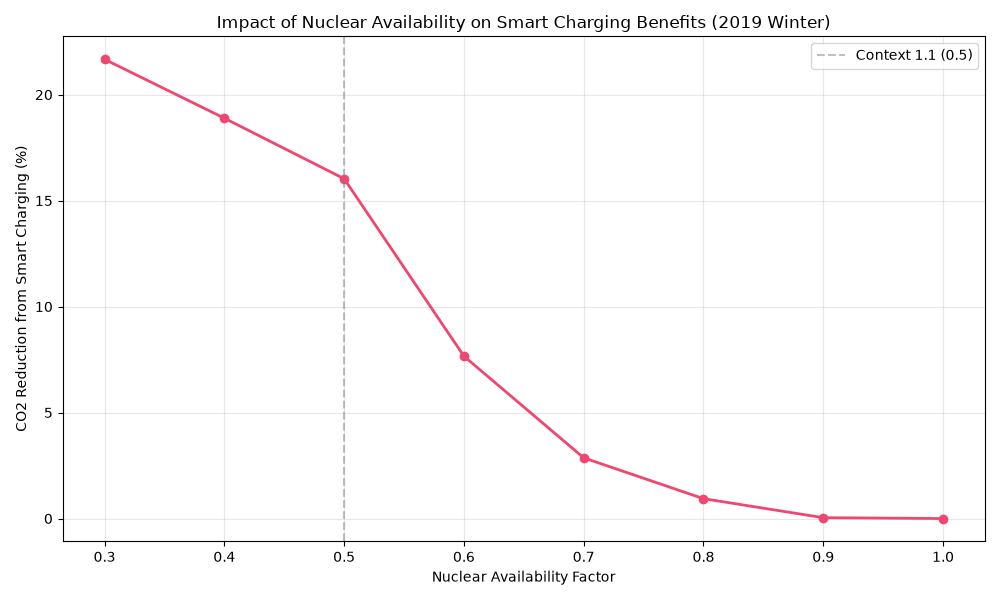
\includegraphics[width=0.86\linewidth]{nuclear_sensitivity.png}
\caption{Impact of nuclear availability on BRD relative gains (2019 winter).}
\label{fig:nuclear_sensitivity}
\end{figure}
\FloatBarrier


\section{Discussion and Realism}
\label{sec:discussion}

\subsection{Scaling and Mean-Field Interpretation}
\label{subsec:scaling_meanfield}

\begin{figure}[H]
\centering
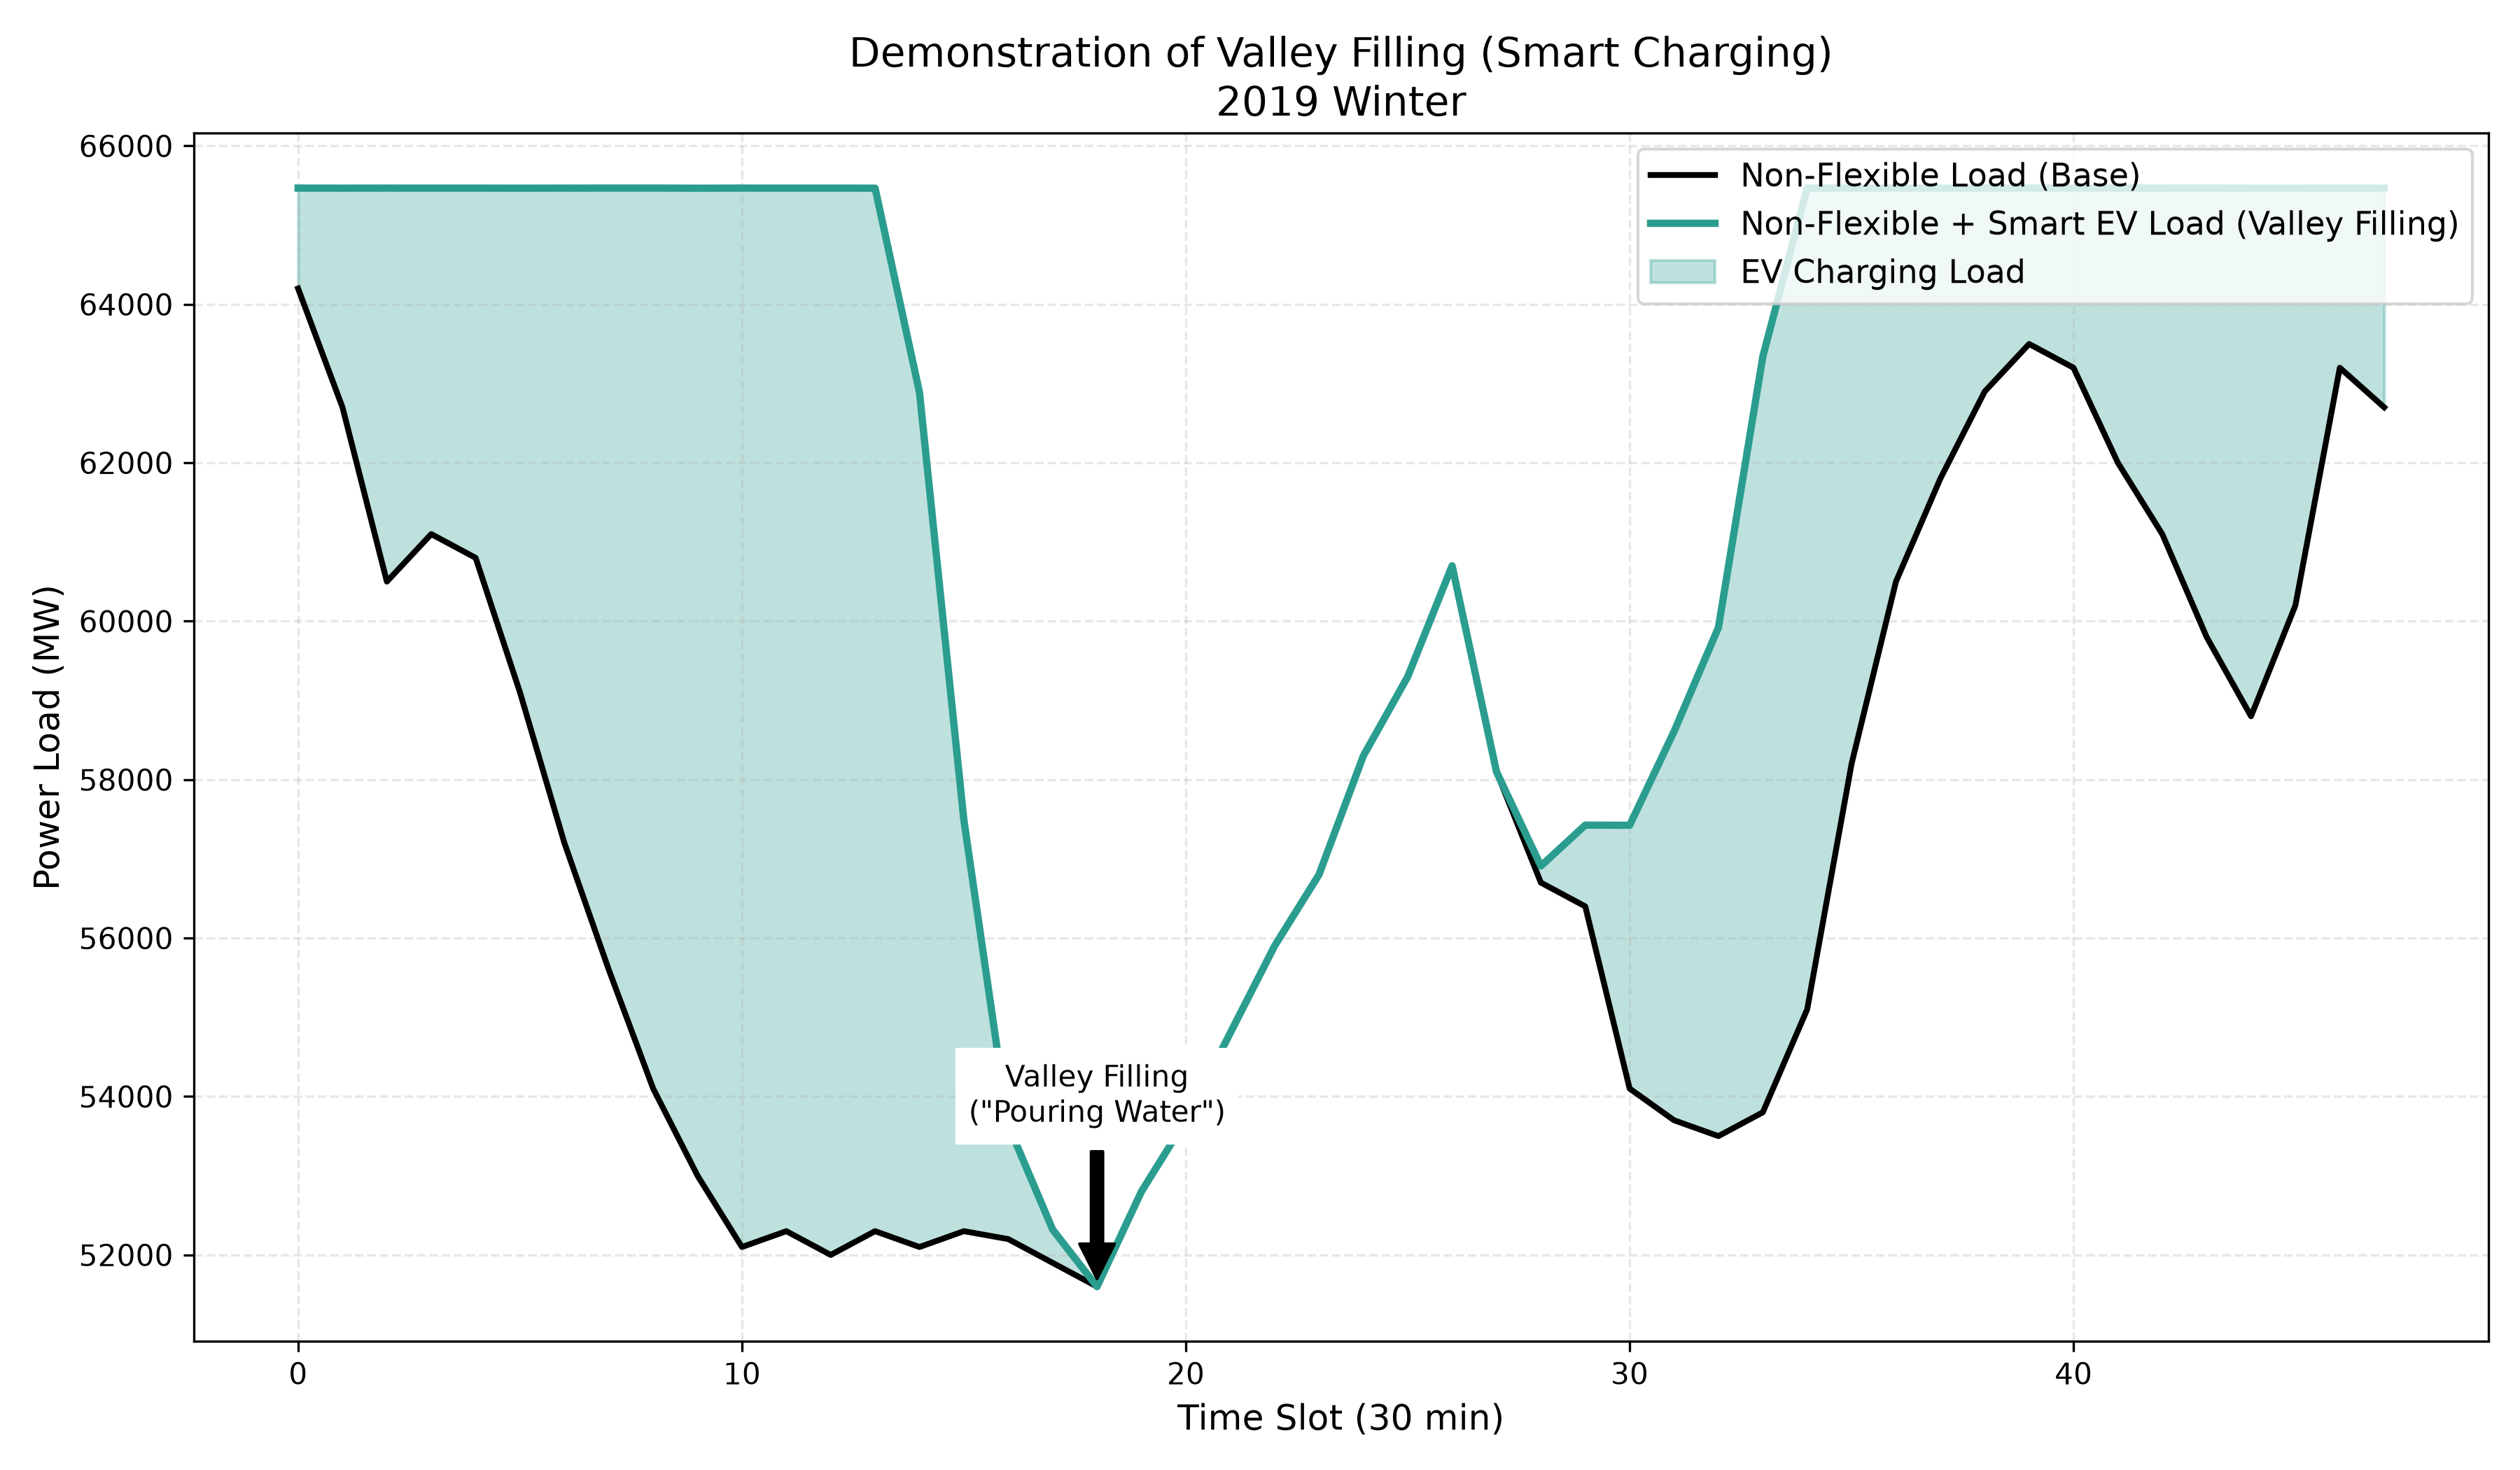
\includegraphics[width=0.90\linewidth]{valley_filling_demo.png}
\caption{Mean-field valley-filling interpretation.}
\label{fig:valley_filling_demo}
\end{figure}

The national profile is obtained from the simulated profile through
\[
\ell^{\mathrm{national}}(t)=\frac{15{,}000{,}000}{500}\,\ell^{\mathrm{sim}}(t).
\]
This scaling is justified by a mean-field view: each EV has negligible unilateral impact and reacts to aggregate signals. Figure~\ref{fig:valley_filling_demo} illustrates how decentralized best responses create a collective valley-filling pattern even though each agent solves only a local constrained problem.

\subsection{Practical Deployment of Policies}
\label{subsec:deployment_policies}

Plug-and-Charge is the easiest to deploy: no communication, no forecasting, no coordination logic. Its limitation is structural: it amplifies local temporal synchronization around arrival times and yields higher system peaks and emissions.

Off-Peak tariff control is also simple to communicate and can be rolled out through existing tariff instruments. However, fixed clock-time incentives create herding behavior: many EVs react to the same temporal signal, so demand concentration is displaced rather than removed. The rebound behavior observed in results, most visible in the synchronized OP-22 variant, is a direct consequence of this synchronized response.

BRD-based smart charging has higher implementation requirements. It needs periodic aggregate signals, iterative updates, and digital control capabilities at charging endpoints. In return, it avoids hard synchronization, uses flexibility windows more efficiently, and delivers lower CO$_2$ scores together with improved peak control. In this sense, BRD trades implementation complexity for robustness of system-level outcomes.

\subsection{Limits of the Approximation}
\label{subsec:model_limitations}

The model is intentionally simplified. Real dispatch follows Unit Commitment with binary on/off constraints, startup costs, minimum up/down times, reserve constraints, and ramping limits. Hence the convex piecewise-linear $f_{\mathrm{CO}_2}$ is a tractable approximation rather than a full operational simulator. The results should be interpreted as structurally informative: they identify robust directional effects (benefit of coordination, rebound risk of synchronized policies, sensitivity to generation mix) rather than exact day-ahead operational forecasts.

\section{Conclusion}
\label{sec:conclusion}

This report addresses the main study questions with a unified theoretical and numerical analysis.
\begin{enumerate}
\item Under the convex piecewise-linear emission model and Cartesian feasibility sets, the decentralized game is an exact potential team game. With exact best responses, equilibria are globally optimal in objective value (PoA$=1$), while charging profiles may be non-unique.
\item The single-EV optimization admits a Water-Filling solution structure, and the BRD coordination loop converges quickly in the tested cases (3 to 7 sweeps).
\item Across the four evaluated scenarios, BRD is never worse than the baselines in CO$_2$ score; gains are largest in winter conditions, and OP and BRD are equal at reported precision in 2019 summer.
\item Load-shape and threshold analyses show that BRD reduces synchronization effects, keeps peak amplification low, and avoids gas-threshold exceedance in the reported scenarios.
\item Sensitivity results confirm that smart-charging gains decrease as nuclear availability increases. The results remain an approximation based on merit-order piecewise modeling rather than a full unit-commitment simulator.
\end{enumerate}

\clearpage
\appendix
\section{Merit-Order Context and CO$_2$ Function}
\label{app:merit_order}
\lstinputlisting[
  style=pycode,
  caption={Model context and piecewise-linear CO$_2$ evaluation (\texttt{smart\_charging.py}, lines 20--86).},
  firstline=20,
  lastline=86
]{../smart_charging.py}

\section{Data Interface and Policy Defin.}
\label{app:data_policy}
\lstinputlisting[
  style=pycode,
  caption={Scenario loading and policy definitions (\texttt{smart\_charging.py}, lines 134--291).},
  firstline=134,
  lastline=291
]{../smart_charging.py}

\section{Scoring and BRD Coordination}
\label{app:scoring_brd}
\lstinputlisting[
  style=pycode,
  caption={CO$_2$ scoring and BRD loop (\texttt{smart\_charging.py}, lines 502--539).},
  firstline=502,
  lastline=539
]{../smart_charging.py}

\end{document}
